% $Id: rfssample.tex,v 19:a118fd22993e 2013/05/24 04:57:55 stanton $
\documentclass[11pt]{article}

% DEFAULT PACKAGE SETUP

\usepackage{setspace,graphicx,epstopdf,amsmath,amsfonts,amssymb,amsthm,versionPO}
\usepackage{marginnote,datetime,enumitem,subfigure,rotating,fancyvrb}
\usepackage{hyperref,float}
\usepackage[longnamesfirst]{natbib}
\usdate

% Make subsubsections inline with a period after the title
\usepackage{titlesec}
\newcommand{\periodafter}[1]{#1.}
\titleformat{\subsubsection}[runin]
{\normalfont\bfseries}{\thesubsubsection}{1em}{\periodafter}

% These next lines allow including or excluding different versions of text
% using versionPO.sty

\excludeversion{notes}		% Include notes?
\includeversion{links}          % Turn hyperlinks on?

% Turn off hyperlinking if links is excluded
\iflinks{}{\hypersetup{draft=true}}

% Notes options
\ifnotes{%
\usepackage[margin=1in,paperwidth=10in,right=2.5in]{geometry}%
\usepackage[textwidth=1.4in,shadow,colorinlistoftodos]{todonotes}%
}{%
\usepackage[margin=1in]{geometry}%
\usepackage[disable]{todonotes}%
}

% Allow todonotes inside footnotes without blowing up LaTeX
% Next command works but now notes can overlap. Instead, we'll define 
% a special footnote note command that performs this redefinition.
%\renewcommand{\marginpar}{\marginnote}%

% Save original definition of \marginpar
\let\oldmarginpar\marginpar

% Workaround for todonotes problem with natbib (To Do list title comes out wrong)
\makeatletter\let\chapter\@undefined\makeatother % Undefine \chapter for todonotes

% Define note commands
\newcommand{\smalltodo}[2][] {\todo[caption={#2}, size=\scriptsize, fancyline, #1] {\begin{spacing}{.5}#2\end{spacing}}}
\newcommand{\rhs}[2][]{\smalltodo[color=green!30,#1]{{\bf RS:} #2}}
\newcommand{\rhsnolist}[2][]{\smalltodo[nolist,color=green!30,#1]{{\bf RS:} #2}}
\newcommand{\rhsfn}[2][]{%  To be used in footnotes (and in floats)
\renewcommand{\marginpar}{\marginnote}%
\smalltodo[color=green!30,#1]{{\bf RS:} #2}%
\renewcommand{\marginpar}{\oldmarginpar}}
%\newcommand{\textnote}[1]{\ifnotes{{\noindent\color{red}#1}}{}}
\newcommand{\textnote}[1]{\ifnotes{{\colorbox{yellow}{{\color{red}#1}}}}{}}

% Command to start a new page, starting on odd-numbered page if twoside option 
% is selected above
\newcommand{\clearRHS}{\clearpage\thispagestyle{empty}\cleardoublepage\thispagestyle{plain}}

% Number paragraphs and subparagraphs and include them in TOC
\setcounter{tocdepth}{2}

% RFS-specific includes:

\usepackage{endnotes}    % Use endnotes instead of footnotes
\usepackage{rfs}          % RFS-specific formatting of sections, etc.
\newcommand{\citeRFS}[1]{\citeauthor{#1}~\citeyear{#1}} % Not very elegant...

% Define theorem-like commands and a few random function names.
\newtheorem{condition}{Condition}
\newtheorem{corollary}{Corollary}
\newtheorem{proposition}{Proposition}
\newtheorem{obs}{Observation}
\newcommand{\argmax}{\mathop{\rm arg\,max}}
\newcommand{\sign}{\mathop{\rm sign}}
\newcommand{\defeq}{\stackrel{\rm def}{=}}

\begin{document}

\setlist{noitemsep}  % Reduce space between list items (itemize, enumerate, etc.)
\onehalfspacing      % Use 1.5 spacing

\newcommand{\tit}{A Sample RFS Paper}

\newcommand{\abs}{There's nothing very interesting here, but the format (achieved using the file \texttt{rfs.sty}) makes it suitable for publication in the \emph{Review of Financial Studies} even if the content doesn't. Here's a nice, informative, double-spaced abstract.}

\title{{\bf \tit}\thanks{We thank\ldots}}

\author{{\bf Richard Stanton} \\
Haas School of Business\\
University of California, Berkeley}

\date{\today}

\maketitle

\newpage

\doublespacing
% Use endnotes instead of footnotes - redefine \footnote command
\renewcommand{\footnote}{\endnote}  % Endnotes instead of footnotes

\centerline{\Large \bf \tit}

\vspace*{1in}

\centerline{\bf Abstract}
\medskip
\abs

\clearpage

Note that RFS doesn't want the first section to be titled.\footnote{Here's a sample footnote (endnote).} Let's put in some sections and subsections to see how they get formatted.

\section{The Model} \label{sec:Model}

There's not actually a model here as it's not really a paper, but this is about where a model might go. 

\subsection{A Subsection}

Nothing very odd about the formatting of section and subsection headings, all defined in \texttt{rfs.sty}. Here's a reference to Section~\ref{sec:subsec} or~\ref{sec:subsub}. Let's also add some parenthetical citations (see~\citeRFS{Stanton:95}, \citeRFS{CarpenterStantonWallace:12}, \citeRFS{Campbell:03}).

{\bf Note:} The formatting at RFS changed some time in the last few years. Previously, for example, RFS used to put a period after the numbers in section and subsubsection headers, but not in subsections. There also used to be no line break after the heading in subsubsections. The current formatting is rather simpler.

To justify adding a subsection here, from now on, we'll assume
\begin{condition}\label{cond:rates}
$0 <  \hat{\mu} < \gamma\sigma^2$.
\vspace{3mm}
\end{condition}
This condition might be useful if there was a model. 

\subsection{Another Subsection, With a Figure}
\label{sec:subsec}

Figures get put at the end, with a note marking where they should go in the text, like this:

\bigskip
\centerline{\bf [Place Figure~\ref{fig:0} about here]}
\bigskip

\subsubsection{A Subsubsection (inline) with a Proposition}
\label{sec:subsub}

Let's put a proposition here.\footnote{The \texttt{titlesec} package is used in the preamble to put the subsubsection heading inline.}
\begin{proposition} \label{prop:3}
If Condition~\ref{cond:rates} is satisfied,  a solution to the central
planner's problem, $V(B,D,t) \in C^2\left( {\mathbb R}_{+}^2 \times
  [0,T] \right)$, with control $a:[0,1]\times[0,T]\rightarrow [-\lambda,\lambda]$
 if  $\gamma>1$ is
\begin{equation} \label{eq:valuea}
V(B,D,t) =  - \frac{(B+D)^{1-\gamma}}{1-\gamma}   w\left(\frac{B}{B+D},t\right).
\end{equation}
\end{proposition}

\clearpage

\noindent {\Large\bf Figure Legends}

\bigskip

\noindent {\bf Figure 1.} \\
{\bf Structure of model: capital can be invested in a bank sector and an equity sector.}  \\
An intermediary has the expertise to reallocate capital between the sectors and to monitor bank capital against bank crashes.

\newpage

\appendix

\section*{An Appendix}
\label{sec:app1}

Here's an appendix with an equation. Note that equation numbering continues from the main body, and RFS does not put a letter before appendix titles, so use the command \verb|\section*| instead of \verb|\section|.
\begin{equation}
  E = mc^2.
\label{eq:eqA}
\end{equation}

\section*{Another Appendix}
\label{sec:app2}

Here's another appendix with an equation.
\begin{equation}
  E = mc^2.
\end{equation}
Note that this is quite similar to Equation~\eqref{eq:eqA}.

\clearpage

% Bibliography

\begin{doublespacing}
\bibliographystyle{rfs}
\bibliography{RHSbib}
\end{doublespacing}

\clearpage

% Print end notes
\renewcommand{\enotesize}{\normalsize}
\begin{doublespacing}
  \theendnotes
\end{doublespacing}

% Figures and tables, showing how to structure captions
\clearpage

\ 
\vfill
\begin{figure}[!htb]
\centerline{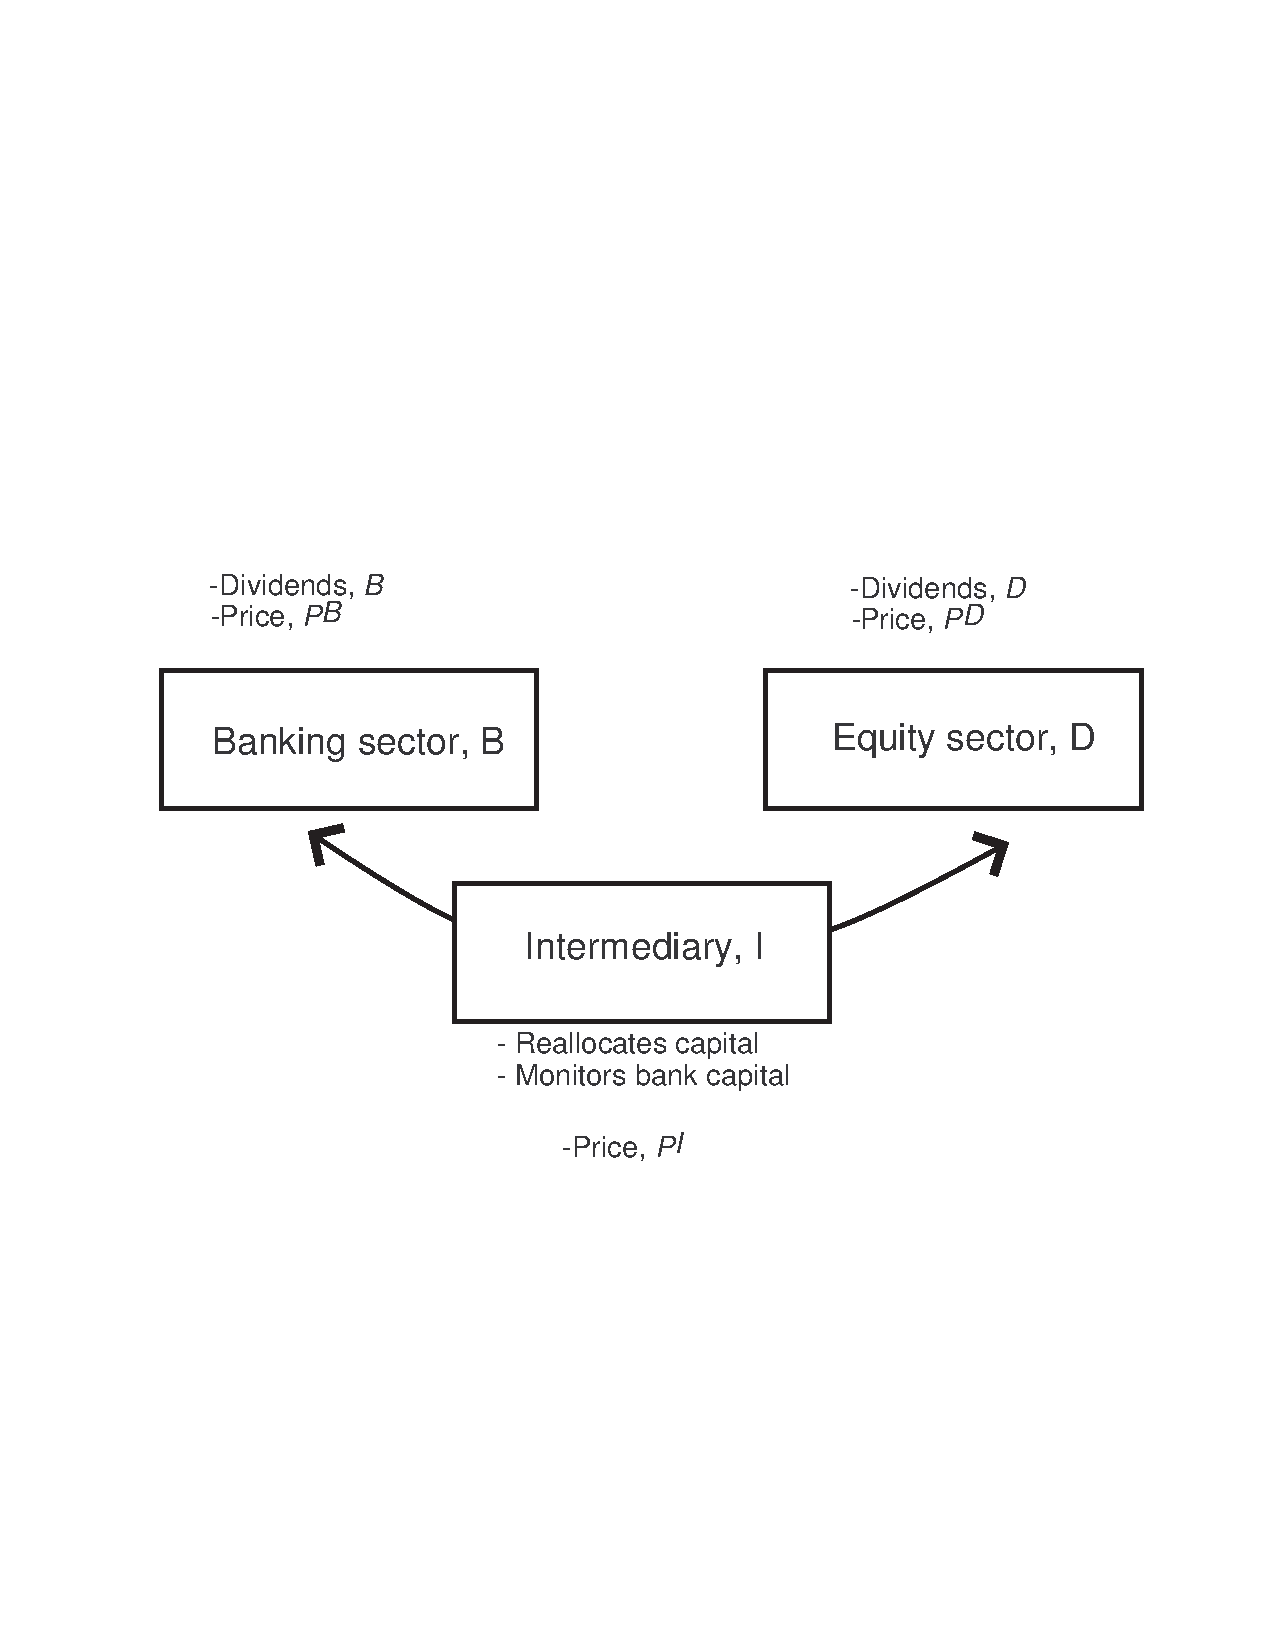
\includegraphics[width=7in]{Figure1}}
\noindent\caption{}
{\bf Structure of model: capital can be invested in a bank sector and an equity sector.} 

An intermediary has the expertise to reallocate capital between the sectors and to monitor bank capital against bank crashes. \label{fig:0}
\end{figure}
\vfill
\ 

\end{document}
